\section{Kontextabgrenzung (JH)}

\subsection{Fachlicher Kontext}
\begin{figure}[H]
	\centering
		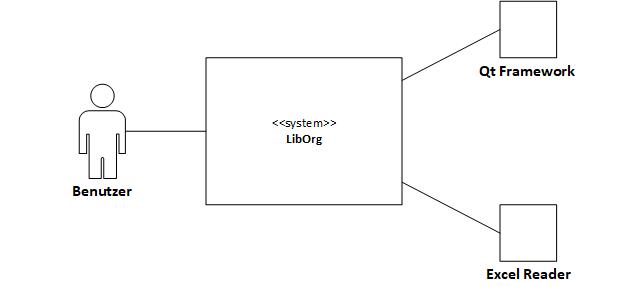
\includegraphics[width=0.50\textwidth]{figures/Fachlicher_Kontext.jpg}
	\caption{Fachlicher Kontext von LibOrg}
	\label{fig:usermanagement}
\end{figure}
\subsubsection{Benutzer}
Das Programm LibOrg dient zur Verwaltung der Bücher und der Ausleihen einer Schulbücherei. Dafür muss ein Benutzer mit dem Programm interagieren und über unterschiedliche Masken Daten mit dem Programm austauschen. Zum Beispiel können neue Bücher hinzugefügt oder ein Buch an einen Schüler ausgeliehen werden.
\subsubsection{QT Framework(Fremdsystem)}
Die GUIs über die der Benutzer mit dem Programm interagiert wurden mithilfe des Qt Frameworks erstellt. Die Verwendung des Qt Frameworks vereinfacht die Erstellung von Benutzeroberflächen.
\subsubsection{Excel Reader(Fremdsystem)}
Um die Schülerdaten aus den vorhanden Excel-Dateien (altes Excel-Format) eilesen zu können wird ein Reader benötigt. Als Excel Reader wurde FreeXL verwendet. 

\subsection{Technischer Kontext}
\begin{figure}[H]
	\centering
		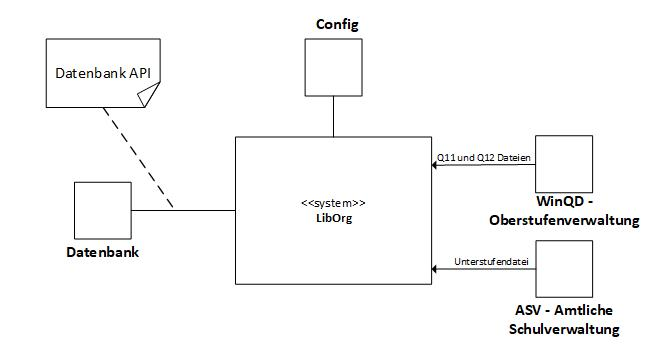
\includegraphics[width=0.50\textwidth]{figures/Technischer_Kontext.jpg}
	\caption{Technische Interaktionen von LibOrg}
	\label{fig:Technischer Kontext}
\end{figure}
\subsubsection{ASV - Amtliche Schulverwaltung}
\label{DEF:ASV}
Aus dem Schülerverwaltungsprogramm der Schule, der ASV - Amtliche Schulverwaltung, werden die Schülerdateien als Excel-Dateien exportiert. Diese Dateien enthalten die Daten der einzelnen Schüler, sowie deren Klassen. Nicht enthalten sind die Kurse von Oberstufenschülern. Es erfolgt kein direkter Zugriff von LibOrg auf ASV.

\subsubsection{WinQD - Oberstufenverwaltung}
\label{DEF:WINQD}
Für die Oberstufe werden die Daten aus dem Programm WinQD exportiert. Hierbei wird jeweils für die Q11 und die Q12 eine Datei erzeugt. Diese enthält die Kurse des aktuellen Schuljahres der Schüler. Auch hier erfolgt kein direkter Zugriff von LibOrg auf WinQD.

\subsubsection{Konfiguration}
Die grundlegenden Einstellungen des LibOrg Programms, wie die gewünschte Hintergrundfarbe, die Abkürzungen der Schulfächer, oder auch der zuletzt angemeldete Benutzer, werden in einer Konfigurationsdatei gespeichert. Diese wird immer zu Beginn des Programms gelesen und die Einstellungen in die Anwendung übernommen. Wenn die Einstellungen geändert werden, werden diese in die Konfigurationsdatei geschrieben, damit sie beim nächsten Programmstart zur Verfügung stehen.

\subsubsection{Datenbank}
Zur Speicherung aller anfallenden Daten des Programms wird eine SQLite Datenbank verwendet. Auf diese wird ausschließlich über eine eigens für die Datenbank geschriebene API zugegriffen. Die API stellt die einheitliche Speicherung, sowie den ordnungsgemäßen Zugriff auf die Datenbank sicher. 